\section{Schematy różnicowe dla zadań dyfuzyjnych}

Będziemy korzystać z równania:

\[
\begin{cases}
\vspace{0.1cm} 
\hspace{0,1cm} \dfrac{\delta \psi}{\delta t} = D\dfrac{\delta^2 \psi}{\delta x^2} \hspace{1cm}, \Omega = [0,L]x[0,\infty] \\
\vspace{0.1cm}
\hspace{0,1cm}\psi_{(x,t)}|_{x=0} = 0 \hspace{0.8cm},t>0 \\
\vspace{0.1cm} 
\hspace{0,1cm}\psi_{(x,t)}|_{x=L} = 0 \hspace{0.7cm},t>0 \\
\vspace{0.1cm} 
\hspace{0,1cm}\psi_{(x,t)}|_{t=0} = \varphi(x) \hspace{0.3cm},x\in[0,L]
\end{cases}
\]

\subsection{Cel ćwiczenia}

Naszym zadaniem było stworzenie algorytmu rozwiązującego następujące równanie:

\[
\begin{cases}
\vspace{0.1cm} 
\hspace{0,1cm} \dfrac{\delta \psi}{\delta t} = D\dfrac{\delta^2 \psi}{\delta x^2} \\
\vspace{0.1cm}
\hspace{0,1cm}\psi|_{x=0} = 0 \\
\vspace{0.1cm} 
\hspace{0,1cm}\psi|_{x=L} = 0 \\
\vspace{0.1cm} 
\hspace{0,1cm}\psi|_{t=0} = sin(\frac{\pi x}{2})
\end{cases}
\]

, gdzie:

$\Omega = [0,2]x[0,1]$
\newline
$D=1$
\newline
\vspace{0.2cm}
$\psi_{analityczna}=\psi(x,t)=sin\Big(\dfrac{\pi x}{2}\Big)e^{-\Big(\dfrac{\pi^2 t}{4}\Big)}$

\subsection{Schemat FTCS}

FTCS (ang. Forward Time Central Space) czyli schemat "w przód":

$$\dfrac{\delta \psi}{\delta t} = D\dfrac{\delta^2 \psi}{\delta x^2}$$

Dla lewej strony równania zastosujemy schemat "w przód", natomiast dla prawej schemat centralny.

Mamy więc:

$$\dfrac{\psi^{(n+1)}_{i}-\psi^n_{i}}{\Delta t}=D\dfrac{\psi^{n}_{i+1}-2\psi^n_{i}+\psi^n_{i-1}}{\Delta x^2}$$

Stąd:

$$\psi^{(n+1)}_{i}=\dfrac{D\Delta t}{\Delta x^2}\Big(\psi^{n}_{i+1}-2\psi^{n}_{i}+\psi^{n}_{i-1}\Big)+\psi^{n}_{i} + O(\Delta t)+O(\Delta x^2)$$

Jest to schemat jawny, warunkowo stabilny, a więc parametry siatki muszą zostać dobrane we właściwy sposób.

Warunkiem stabilności dla takiego zadania jest następująca relcja:

$$\dfrac{D\Delta t}{\Delta x^2}\le \dfrac{1}{2}$$

\subsection{Algorytm}

//kod ftcs

\subsection{Wykresy}

Dla n = 5:

{\centering
	
	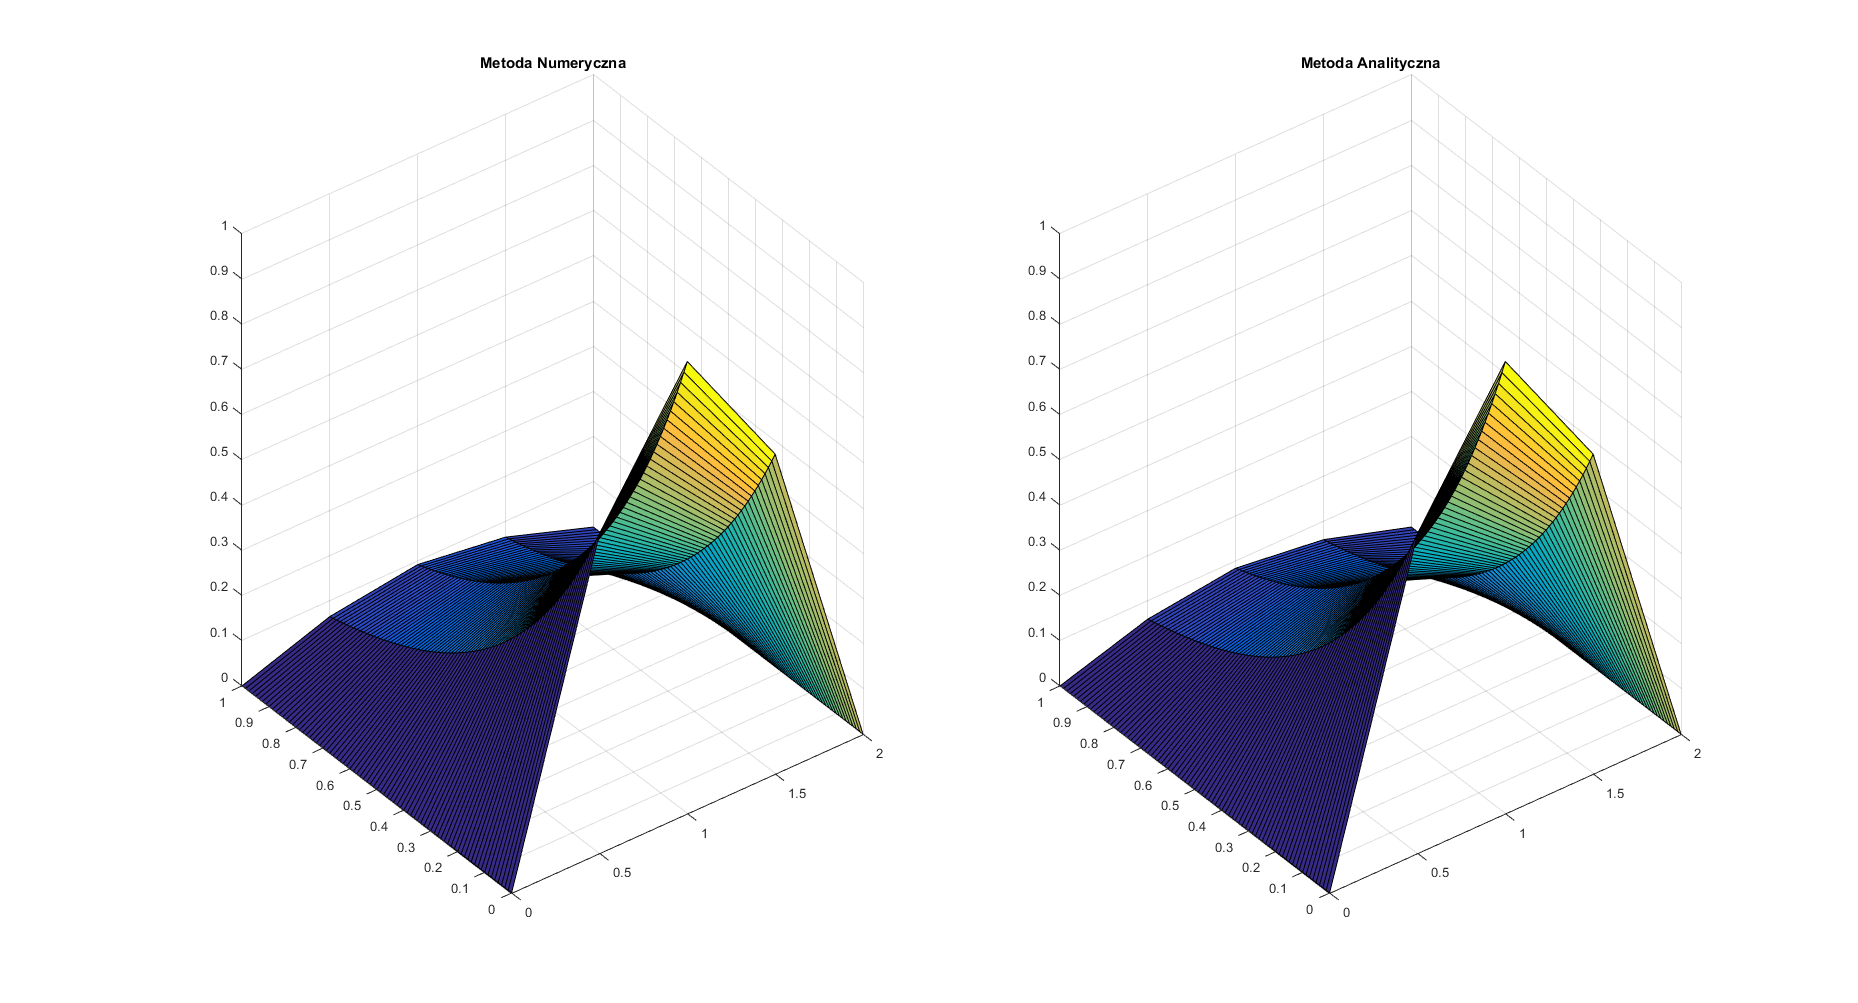
\includegraphics{Lab7/charts/ftcs/5.png}
	
}

Liczba wykonanych iteracji $ = 80 $

Czas wykonywania algorytmu $ = 0.100 s$

Dla n = 10:

{\centering
	
	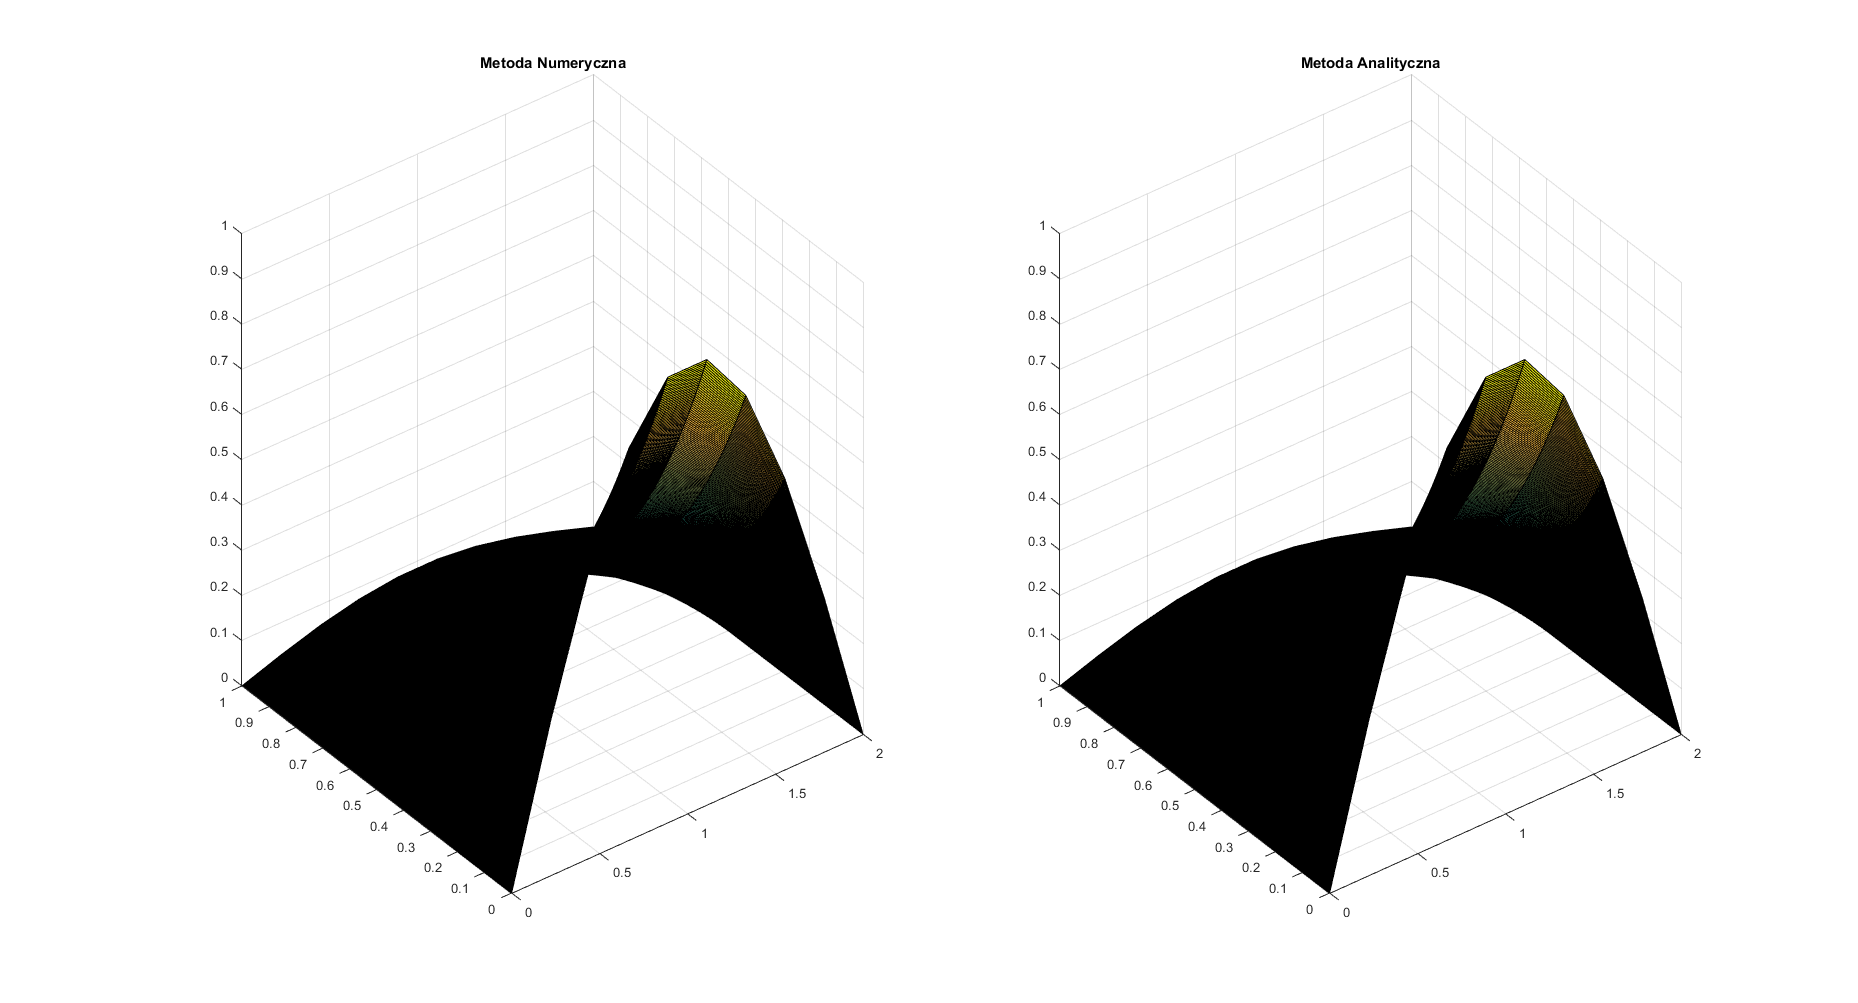
\includegraphics{Lab7/charts/ftcs/10.png}
	
}

Liczba wykonanych iteracji $ = 405 $

Czas wykonywania algorytmu $ = 0.163 s$

\newpage

Dla n = 15:

{\centering
	
	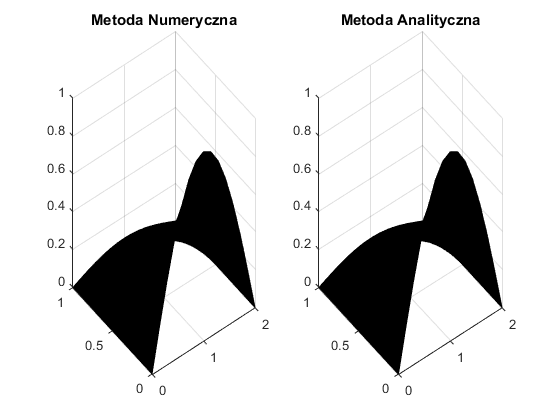
\includegraphics{Lab7/charts/ftcs/15.png}
	
}

Liczba wykonanych iteracji $ = 980 $

Czas wykonywania algorytmu $ = 0.192 s$

Dla n = 30:

{\centering
	
	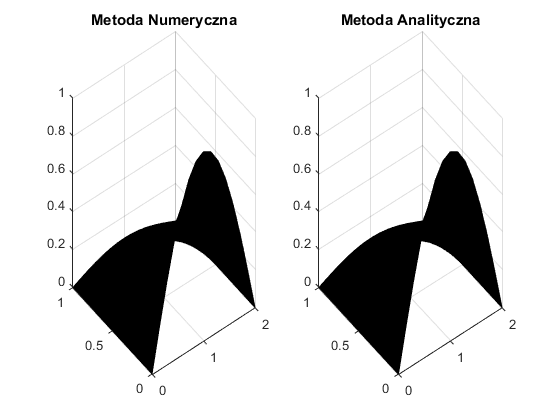
\includegraphics{Lab7/charts/ftcs/15.png}
	
}

Liczba wykonanych iteracji $ = 4205 $

Czas wykonywania algorytmu $ = 0.472 s$

\subsection{Schemat BTCS}



